\title{\vspace{160px} \textbf{\huge{Telecommunication Theory}} \\\vspace{17.5px} \LARGE{Lab report 2}  \vspace{10px}}
\author{Alessandro Trigolo}
\date{September 18, 2023}

\begin{document}
\maketitle \newpage


\section*{Objective}\label{objective}
The goal of the laboratory is to observe the effect produced by the \textit{Gaussian White Noise} (\textbf{GWN}) during a data transmission. Initially, a data set is provided and then it is converted to a signal. The GWN will be added to the signal for the purpose of simulating the disturbance during a transmission and finally, the received signal will be detected. There will be two types of modulation of the signal: the first one will not modify the signal at all meanwhile the second one, called \textit{Non-Return to Zero} (\textbf{NRZ}), will invert and amplify the signal in order to reduce the impact of the GWN. During this phase, it is possible to notice the difference that the \textit{Signal to Noise Ratio} (\textbf{SNR}) makes during the transmission and how important it is to choose the modulation of a signal.

% 
% 
\section*{Source code and plots} \label{source_code_plots}
The MatLab source code produced in order to accomplish the laboratory goal is presented in the following section. Next to the lines of code, there will be some explanatory comments for the purpose of making the source code more readable. The code is divided into tasks and, at the end of each, it is presented the plot produced.

\lstset{style = MatLab}

\subsection*{Task 1}
In the first task, it was requested to create a random sequence of "\texttt{1}" and "\texttt{0}" and then display the sequence as a discrete plot. In this particular case the number of "\texttt{1}" and "\texttt{0}" is stored in the variable \texttt{N} which is set to \texttt{10}. Noticeably, due to the fact that the random sequence is re-calculated every time the code is run, in the report, as a reference, it is used the fixed sequence: \texttt{[ 0, 1, 1, 0, 0, 0, 1, 0, 1, 1 ]}.

\begin{lstlisting}
clc, clearvars, clear

% --- 1: creating the dataset

N = 10; % numbers of bits

index = randi(2, N, 1); % randomly generated indexes
arr=[0,1]; % creates small array
s = arr(index); % vector of random 0s and 1s

figure(1) % creates the figure
subplot(3, 2, 1), stem(s, "b", "Linewidth", 1) % draws the function and puts it on the figure
grid on; % adds grids
xlabel("Sample No."), ylabel("Sample Values"), title("Initial data") % adds labels and title
ylim([-.5, 1.5]); % adjusts Y-axes   
\end{lstlisting}
% 
\begin{figure}[h!]
    \centering
    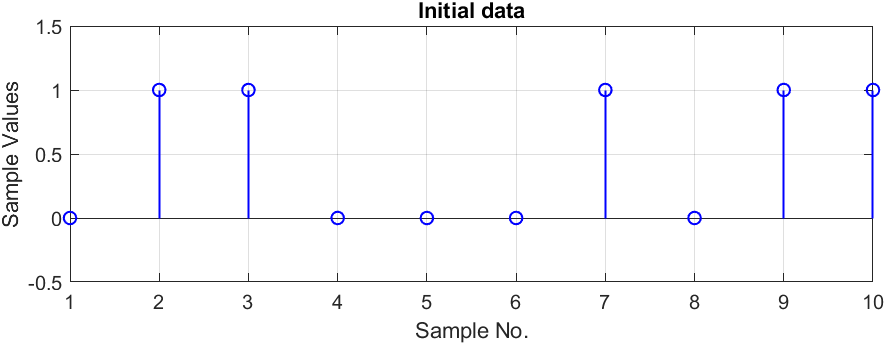
\includegraphics[width = .8\textwidth]{lab-1/imgs/initial_data.png}
\end{figure}

% 
\subsection*{Task 2}
The second task requested to convert the discrete signal into unipolar pulses with an amplitude of 1 Volt. In order to do that it has been used the \textit{Kroner} multiplication that simulates the \textit{Digital to Analogic Conversin} (\textbf{DAC}).
\begin{lstlisting}
% --- 2: conversion of the discrete signal

SC = ones(1, 100); 
sTx = kron(s, SC); % kroner multiplication, utilized to perform DAC

subplot(3, 2, 2), plot(sTx, "b", "Linewidth", 1);
grid on;
xlabel("Time, units"), ylabel("Signal"), title("Converted signal");
ylim([-.5, 1.5]);
\end{lstlisting}

\begin{figure}[h!]
    \centering
    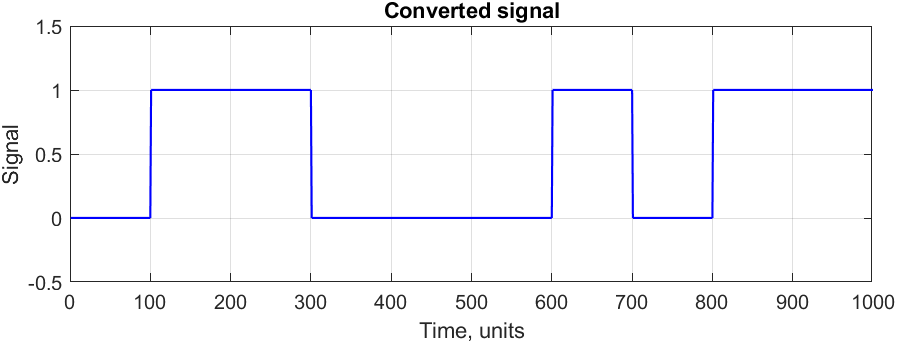
\includegraphics[width = .8\textwidth]{lab-1/imgs/converted_signal.png}
\end{figure}

% 
\subsection*{Task 3}
Task number three asked to introduce the GWN to the converted signal. For the purpose of doing that, a new signal has been created with the \texttt{awgn} function which added the GWN to the signal with a \texttt{SNR} set to \texttt{20}: this means that the transmitted signal is 100 times stronger than the GWN. After plotting the disturbed signal it was added a red line indicating the threshold utilized in Task 4.

\begin{lstlisting}
% --- 3: addition of GWN to the signal

% Signal to Noise Ratio
% i.e. SNR = 20 --> signal is 100 times stronger than the noise
SNR = 20; % dB

sRx = awgn(sTx, SNR); % awgn = Additive White Gaussian Noise

subplot(3, 2, 3), plot(sRx, "b");
grid on;
xlabel("Time, units"), ylabel("Signal"), title("Signal with GWN");
ylim([min(sRx), max(sRx)]);

threshold = ( max(sTx) + min(sTx) ) / 2; % calculates the threshold
hold on, plot([0, length(sTx)], [threshold, threshold], "r", "Linewidth", 1), hold off; % adds threshold red line
\end{lstlisting}

\begin{figure}[h!]
    \centering
    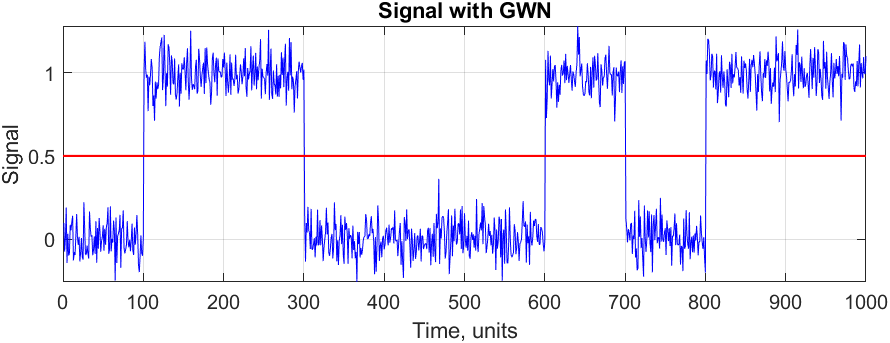
\includegraphics[width = .8\textwidth]{lab-1/imgs/noise_SNR20.png}
\end{figure}

% 
\subsection*{Task 4}
The fourth task requested to regenerate the received disturbed signal into a pulse signal like the one shown in Task 2. In order to accomplish the detection it is sufficient to introduce a threshold in the middle of the disturbed signal: ideally, the threshold has a value of 0.5 V. The detection algorithm is very simple to make: if the value of the disturbed signal is greater than the threshold then the regenerated signal will have the value "\texttt{1}", else it will have the value "\texttt{0}".

\begin{lstlisting}
% --- 4: Detection signal with GWN

% detects signal
%   signal > threshold --> 1
%   signal < threshold --> 0
sDt = sRx > threshold;

subplot(3, 2, 4), plot(sDt, "r", "Linewidth", 1);
grid on;
xlabel("Time, units"), ylabel("Signal"), title("Signal detection");
ylim([-.5, 1.5]);
\end{lstlisting}
% 
\begin{figure}[h!]
    \centering
    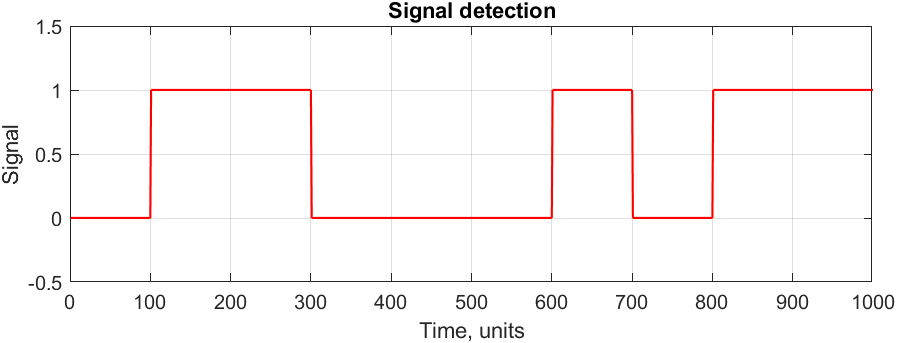
\includegraphics[width = .8\textwidth]{lab-1/imgs/noise_detection_SNR20.png}
\end{figure}

% 
\subsection*{Task 5}
Comparing the plot in Task 4 and the plot in Task 2 it is noticeable that there are no differences at all. This means that using a signal 100 times stronger than the GWN is a synonym for a good transmission because no errors have occurred during the detection.

\begin{figure}[h!]
    \centering
    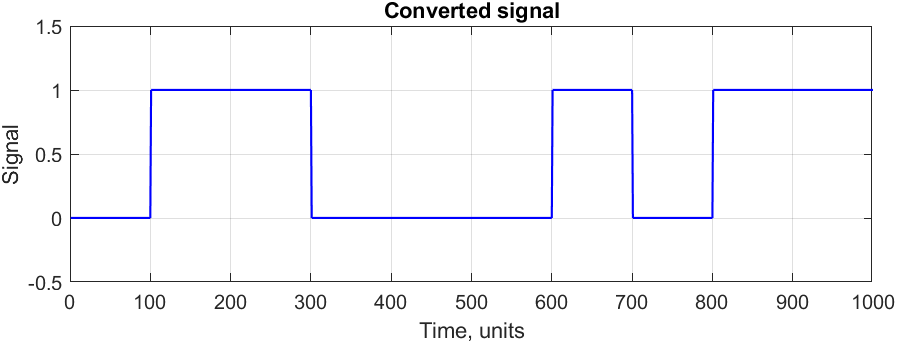
\includegraphics[width = .6\textwidth]{lab-1/imgs/converted_signal.png}
    \vspace{10 px}
    
    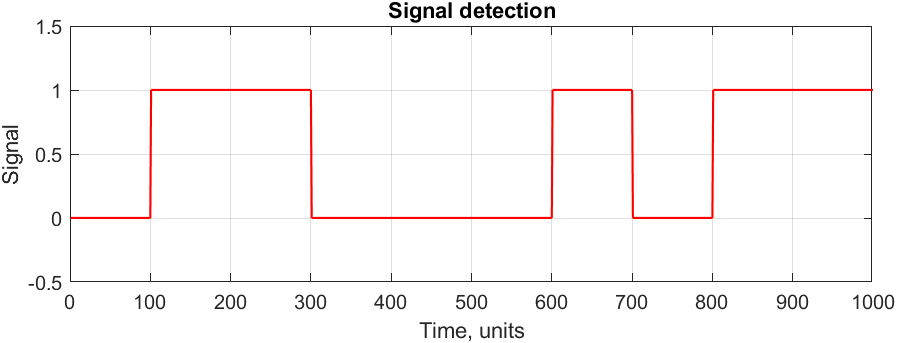
\includegraphics[width = .6\textwidth]{lab-1/imgs/noise_detection_SNR20.png}
\end{figure}

% 
\subsection*{Task 6}
Task 6 asked to decrease the SNR from 20 to 10 meaning that now the transmitted signal is only 10 times stronger than the GWN. The source code is identical to the one shown in the previous task with the obvious exception that the \texttt{SNR} variable is now set to 10 instead of 20. 

By only looking at the new disturbed signal it is possible to conclude that the detection won't detect the signal properly. That is due to the fact that several parts of the signal are overcoming the threshold because of the GWN even though they shouldn't.
\begin{figure}[h!]
    \centering
    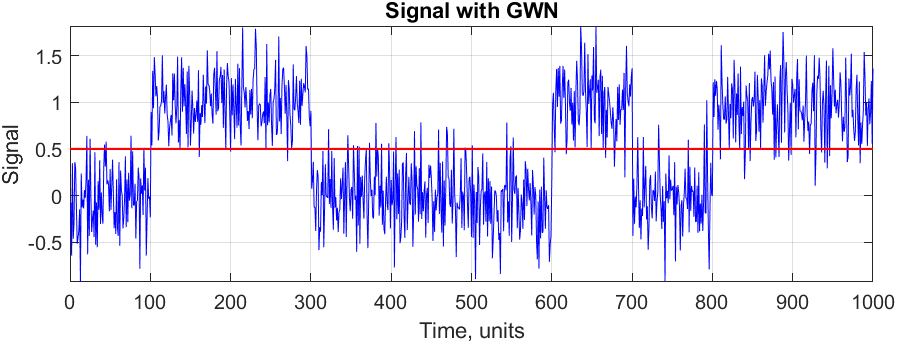
\includegraphics[width = .8\textwidth]{lab-1/imgs/noise_SNR10.png}
\end{figure}

\FloatBarrier\noindent Sure enough, after receiving and detecting the weak disturbed signal, it is harder, almost impossible, to understand what the actual signal was. This means that the transmission is far from optimal because the signal is very weak.

\begin{figure}[h!]
    \centering
    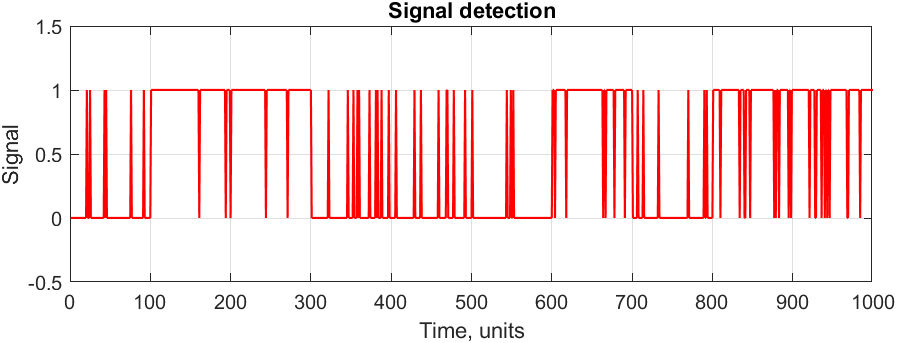
\includegraphics[width = .8\textwidth]{lab-1/imgs/noise_detection_SNR10.png}
\end{figure}

% 
\subsection*{Task 7}
The final task requested to change the type of modulation and redo tasks 3, 4 and 5. The type of modulation chosen is the NRZ (\textit{Non-Return to Zero}) which amplifies and reverses the signal: 1 becomes -1 and 0 becomes 1. In such a way, the overall amplitude (top-bottom) has doubled. To the NRZ modulated signal will be added the GWN and then it will be plotted with the threshold. It is possible to notice that the noise is now more distant from the threshold so it is expected that the newly detected signal won't be as disturbed as the one shown in Task 6.

\begin{lstlisting}
% --- 7: changing modulation of the signal to NRZ

% creates NRZ signal:
%   1 --> -1 
%   0 --> 1
sTx = (-2 * sTx) + 1; 

sRx = awgn(sTx, SNR); % awgn = Additive White Gaussian Noise

subplot(3, 2, 5), plot(sRx, "b");
grid on;
xlabel("Time, units"), ylabel("Signal"), title("NRZ signal with GWN");
ylim([min(sRx), max(sRx)]);

threshold = ( max(sTx) + min(sTx) ) / 2; % recalculates the threshold 
hold on, plot([0, length(sTx)], [threshold, threshold], "r", "Linewidth", 1), hold off; % adds threshold red line
\end{lstlisting}

\begin{figure}[h!]
    \centering
    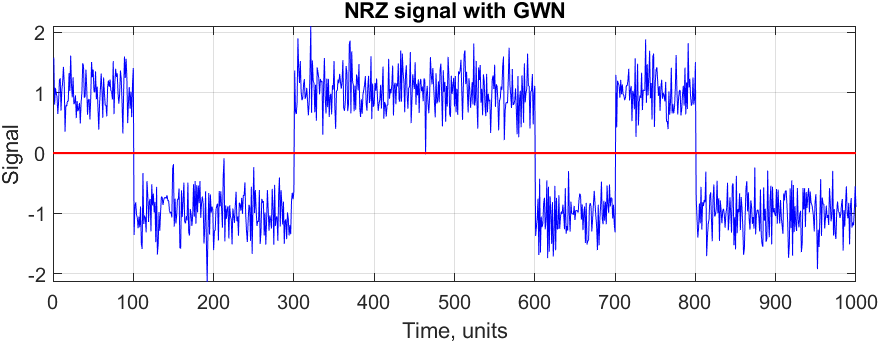
\includegraphics[width = .8\textwidth]{lab-1/imgs/NRZ_SNR10.png}
\end{figure}

\noindent After plotting the disturbed signal it is necessary to detect and regenerate the original transmitted signal. The NRZ signal, as previously mentioned, is reversed so the detection algorithm has to reverse back to the original: if the NRZ signal is lower than the threshold then the signal is restored to 1, else it is restored to 0.

\begin{lstlisting}
% detects signal
%   signal < threshold --> 1
%   signal > threshold --> 0
sDt = sRx < threshold;

subplot(3, 2, 6), plot(sDt, "r", "Linewidth", 1);
grid on;
xlabel("Time, units"), ylabel("Signal"), title("Signal detection");
ylim([-.5, 1.5]);
\end{lstlisting}

\begin{figure}[h!]
    \centering
    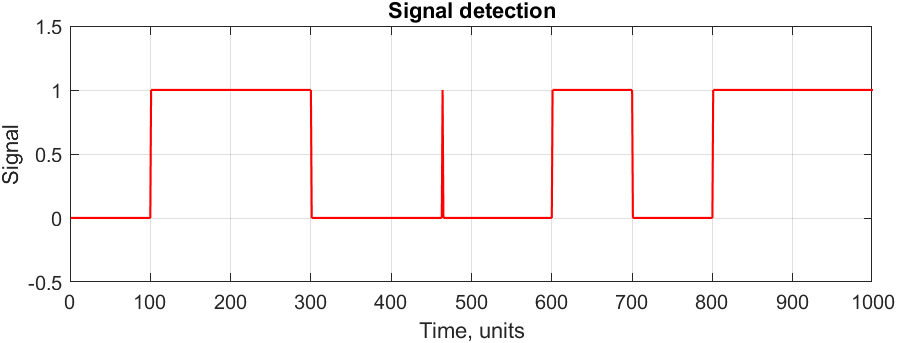
\includegraphics[width = .8\textwidth]{lab-1/imgs/NRZ_detection_SNR10_1.png}
\end{figure}

\noindent The newly detected signal is almost identical to the transmitted one. Precisely because the GWN follows a Gaussian distribution, after running the code sometimes, if we are lucky enough, it is possible to get the detected signal completely identical to the initial one, without any errors.

\begin{figure}[h!]
    \centering
    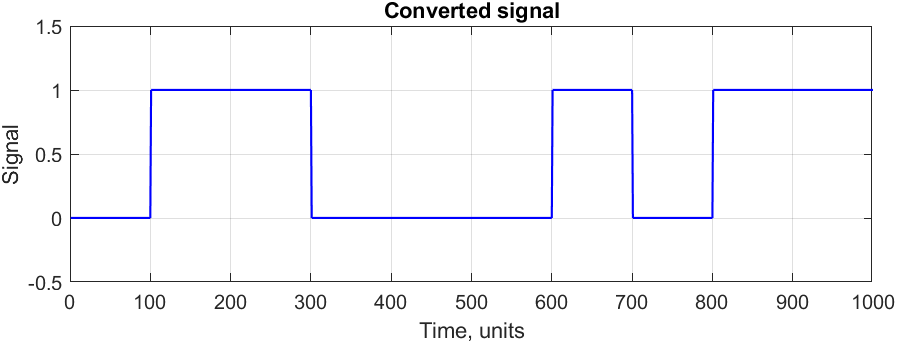
\includegraphics[width = .6\textwidth]{lab-1/imgs/converted_signal.png}
\end{figure}

\begin{figure}[h!]
    \centering
    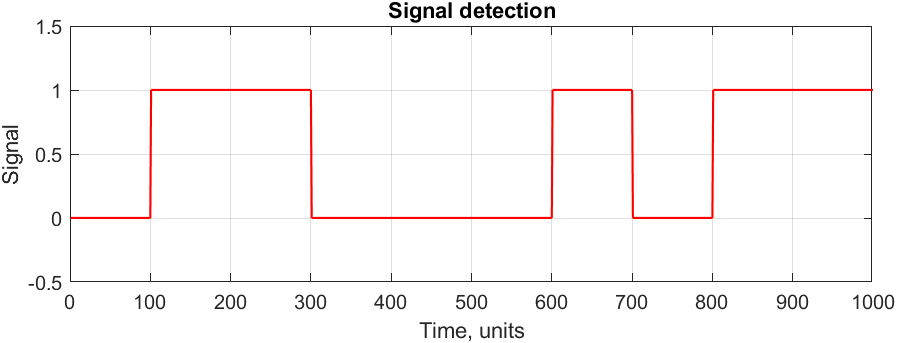
\includegraphics[width = .6\textwidth]{lab-1/imgs/NRZ_detection_SNR10_2.png}
\end{figure}

% 
% 
\section*{Conclusions}\label{conclusions}
Through these simulations, we can conclude that the NRZ modulation of the signal is more reliable because the signal is not affected by the Gaussian White Noise even though the signal's energy is not significantly higher than the energy of the noise. This means that the NRZ modulation of the signal increases the success rate of the transmission thanks to the doubled signal amplitude. If the signal is strong enough (i.e., 100 or 1000 times more powerful than the GWN) by observing the simulations, it is possible to conclude that not modulating the signal is sufficient to have a successful transmission but, clearly, the simulations do not represent a real transmission because, other than the GWN, there could be different types of disturbances that could be stronger than the GWN so, consequently, it is always better to modulate the signal. 



\end{document}